\clearpage\NoSourceHead\SourceLeaf{403}
\SourceGroup{III}
\HistoricTitle{FRAGEN ZUR METAPHYSIK DER MATHEMATIK.}
\HistoricCitation{[Aus Handbuch 19, Be, Kleine Aufsätze aus verschiedenen Theilen der Mathematik, Angefangen im May 1809, S. 136, 137.]}
\begin{center}1.\end{center}
\noindent\hspace*{\parindent}Welches ist die wesentliche Bedingung, dass eine Verknüpfung von Begriffen als sich auf eine \textls[120]{Grösse} beziehend gedacht werden könne?
\begin{center}2.\end{center}
\noindent\begin{minipage}[t]{.24\linewidth}\vspace{0pt}\centering
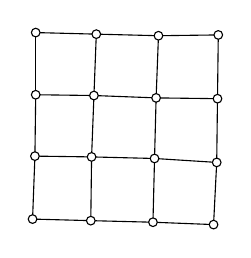
\begin{tikzpicture}[x=.010cm,y=-.010cm,line width=.4pt]
\coordinate (A) at (209,1101);\coordinate (B) at (286,1103);\coordinate (C) at (365,1105);\coordinate (D) at (441,1104);
\coordinate (E) at (209,1180);\coordinate (F) at (283,1181);\coordinate (G) at (362,1184);\coordinate (H) at (440,1185);
\coordinate (I) at (208,1258);\coordinate (J) at (280,1259);\coordinate (K) at (360,1261);\coordinate (L) at (439,1266);
\coordinate (M) at (205,1338);\coordinate (N) at (279,1340);\coordinate (O) at (358,1342);\coordinate (P) at (435,1345);
\foreach \a/\b in {A/B,B/C,C/D,E/F,F/G,G/H,I/J,J/K,K/L,M/N,N/O,O/P,A/E,E/I,I/M,B/F,F/J,J/N,C/G,G/K,K/O,D/H,H/L,L/P}{\draw (\a)--(\b);}
\foreach \p in {A,B,C,D,E,F,G,H,I,J,K,L,M,N,O,P}{\draw[fill=white] (\p) circle[radius=.055cm];}
\end{tikzpicture}
\end{minipage}\hfill\begin{minipage}[t]{.72\linewidth}\vspace{0pt}\setlength{\parindent}{1.2em}
\noindent\hspace*{\parindent}Alles wird viel einfacher, wenn man zuerst von der Unendlichkeit der Theilbarkeit abstrahirt und bloss Discrete Grössen betrachtet. Z. B. wie bei den biquadratischen Resten die Punkte als Gegenstände, die \textls[120]{Übergänge}, also Verhältnisse, als Grössen, wo die Bedeutung von \(a+bi-c-di\) sogleich klar ist.
\end{minipage}\par
\begin{center}[3.]\end{center}
\noindent\hspace*{\parindent}Die Mathematik ist so im allgemeinsten Sinn die Wissenschaft der Verhältnisse, indem man von allem Inhalt der Verhältnisse abstrahirt.

Verhältniss setzt zwei Dinge voraus und heisst dann einfaches Verhältniss etc.
\begin{center}[4.]\end{center}
\noindent\hspace*{\parindent}Die allgemeine Vorstellung von Dingen, wo jedes nur zu zweien ein Verhältniss der Ungleichheit hat, sind Punkte in einer Linie.
\clearpage\SourceLeaf{404}\ArithmeticHead{397}{R}{FRAGEN ZUR METAPHYSIK DER MATHEMATIK.}
\noindent\hspace*{\parindent}Kann ein Punkt zu mehr als zweien ein Verhältniss haben, so ist das Bild davon die Lage von Punkten in einer Fläche, die durch Linien verbunden sind. Soll hier aber eine Untersuchung möglich seyn, so kann sie nur die Punkte betreffen, die zu dreien in einem Wechselverhältniss stehen, und wo es zwischen den Verhältnissen ein Verhältniss gibt.
\begin{center}[5.]\end{center}
\noindent\hspace*{\parindent}Ganz vorzüglich wichtig wird seyn, die Theorie des Gegensatzes zur Klarheit zu bringen ohne \textls[120]{Grösse}. So kommen z. B. beim Nivelliren einer Ebne folgende Gegensätze vor. Die Stellung der Blase in der Glasröhre ist bei der Ruhe bestimmt durch [die] Geometrische Axe der Röhre [und eine] Linie durch die Ebne der Füsse.
\begin{center}BEMERKUNG.\end{center}
{\small\noindent\hspace*{\parindent}Die vorstehende Aufzeichnung folgt unmittelbar auf die in den Werken VIII, S. 444 abgedruckte Bemerkung, die »1825, Dec. 4« datiert ist. Man vergleiche zu dem Gegenstande die \textit{Anzeige} der zweiten Abhandlung über die biquadratischen Reste vom Jahre 1831, Werke II, S. 169, besonders S. 174 ff., ferner den weiter unten im \textit{Briefwechsel} abgedruckten Brief [6.] von \textsc{Gauss} an \textsc{Grassmann} vom 14. Dezember 1844. Zu dem im art. [5.] als Beispiel herangezogenen Nivellieren einer Ebene vergleiche man die Notiz Werke VIII, S. 197.\par}
\begin{flushright}\textsc{Schlesinger}.\end{flushright}
\ClosingRule
